\documentclass[tikz]{standalone}
\usepackage{pgfplots}
\tikzset{
  jumpdot/.style={mark=*,solid},
  excl/.append style={jumpdot,fill=white},
  incl/.append style={jumpdot,fill=black},
}
\usetikzlibrary{arrows.meta}
\pgfplotsset{compat=1.11}
\begin{document}
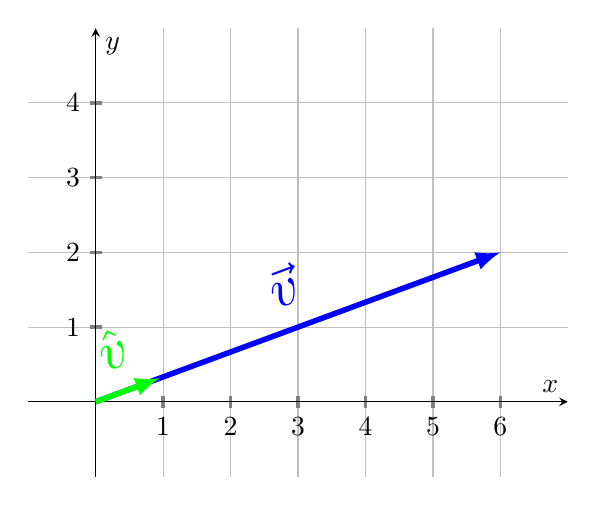
\begin{tikzpicture}
\begin{axis}[
  axis lines=middle,
  grid=major,
  xmin=-1,
  xmax=7,
  ymin=-1,
  ymax=5,
  xlabel=$x$,
  ylabel=$y$,
  xtick={0,1,...,6},
  ytick={0,1,...,4},
  %xticklabel = \empty,
  %yticklabel = \empty,
  tick style={very thick},
  %restrict y to domain = -2:30,
  legend style={at={(rel axis cs:0,1)},anchor=north west,draw=none,inner sep=0pt, fill = white}
]

\draw[line width=2pt, blue, -latex] (0,0) -- (6,2) node[sloped,above, midway,scale = 2] {$\vec{v}$};
\draw[line width=2pt, green, -latex] (0,0) -- (0.949,0.316) node[sloped,above, midway,scale = 2] {$\hat{v}$};

%\addplot[blue,very thick,domain=-5:5,samples=100] gnuplot {x**3 + x**2 - x};
%\draw[green,very thick] (1,0) -- (1,2);
%\draw[green,very thick] (3,0) -- (3,2);
%\draw [dashed] (2,-10) -- (2,40);
%\addplot[incl, draw=blue] coordinates {(-2,3)} node[above] {$f'(x)$ is undefined};
%\addplot[incl, draw=blue] coordinates {(.5,-1.25)} node[below] {$f'(x) = 0$};
%\addplot[incl, draw=blue] coordinates {(3,2)} node[pin={[pin distance = .1cm]180:{$f'(x)$ is undefined}}] {};

%\addplot[excl, draw=blue] coordinates {(-2,0)};


%\addlegendentry{$f(x) = x^3 + x^2 - x$};

\end{axis};
\end{tikzpicture}

\end{document}